\documentclass{beamer}
\usetheme{Madrid}
\usecolortheme{spruce}

\usepackage{pgfplots}

\usepackage{bm}

\usepackage{color}

\usepackage{graphicx}

\graphicspath{{./img/}}

\title{Stochastic Gradient Descent}
\subtitle{STAT 672 Project}
\author{Tom Wallace}
\institute{George Mason University}
\date{Spring 2018}


\begin{document}

\frame{\titlepage}

%%%%%%%%%%%%% Introduction %%%%%%%%%%%%%%

\begin{frame}
	\frametitle{Optimization is everywhere, and sometimes is easy}
	Many statistical procedures involve minimizing or maximizing some function 
	applied to data \\~\\

	In \textbf{parametric} statistics, we often make assumptions that make this optimization ``nice'':
	\begin{itemize}
		\item \small Example: in OLS, we do not need to try
			different values
			of $\hat{\beta}$ to see which minimizes the loss
			function, we (typically) can just evaluate
			$(X'X)^{-1}X'Y$ \\~\\
	\end{itemize}
	\smallskip

	\centering
	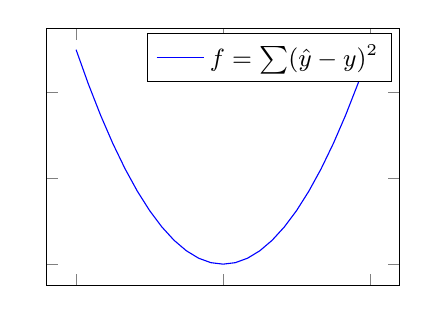
\begin{tikzpicture}
		\begin{axis}[
			yticklabels={,,},
			xticklabels={,,},
			width=0.5\textwidth,
			height=0.4\textwidth,
			legend style = {font=\small}
		]
			\addlegendentry{$f=\sum (\hat{y} - y)^2$}
			\addplot[mark=none, color=blue]{x^2};
		\end{axis}
	\end{tikzpicture}
\end{frame}

\begin{frame}
	\frametitle{Other times, optimization is not so easy}
	Suppose that we have a typical supervised classification problem:
	\begin{itemize}
		\item \small Non-parametric: no assumptions about distribution of data
		\item Feature vector $\mathbf{X}_i$, label $Y_i$
		\item Want to find best prediction function $f_w^*$ from class $\mathcal{F}$
		\item Optimization: pick weights $\bm{w}$ that minimize
			empirical risk according to some convex
			loss function $L(f_w(x), y)$ \\~\\
	\end{itemize}

	Our lack of assumptions requires a different approach to optimization
	\begin{itemize}
		\item \small Cannot analytically identify stationary point
		\item Need to numerically search for it
	\end{itemize}
\end{frame}

\begin{frame}
	\frametitle{Gradient descent is an iterative search procedure}
	\begin{figure}[h]
	\centering
	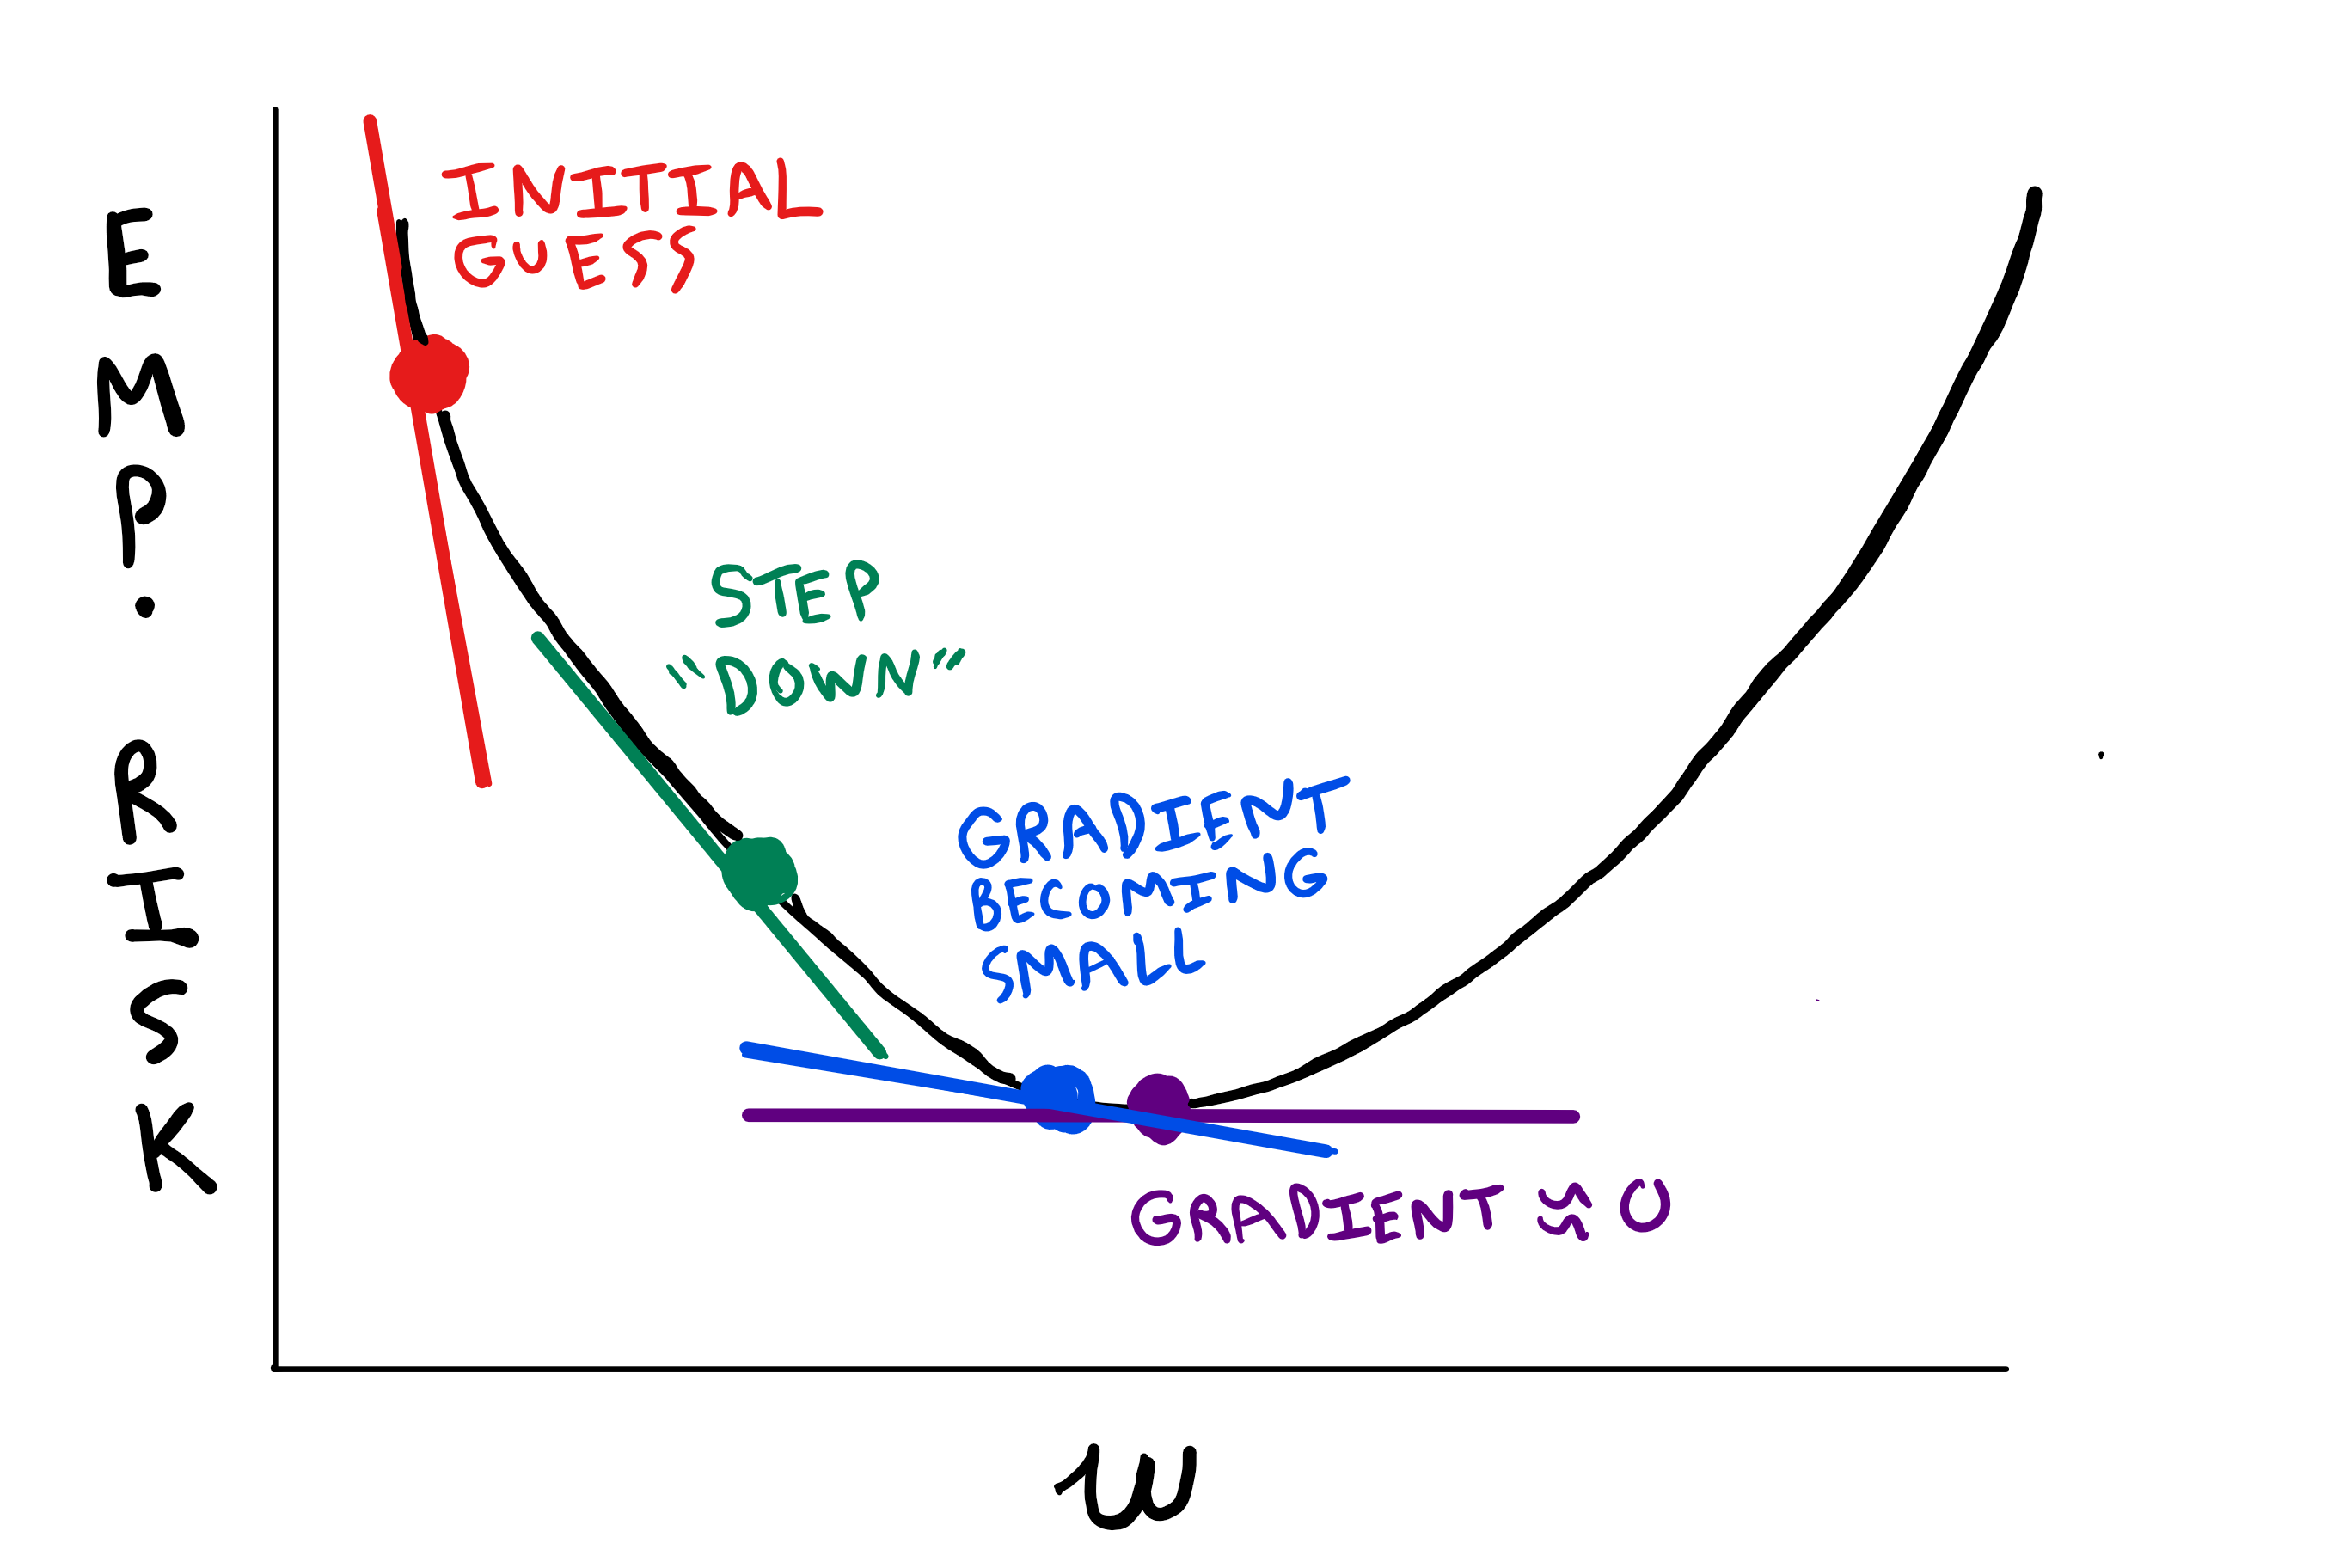
\includegraphics[scale=0.33]{Sketch}
	\end{figure}
\end{frame}

\begin{frame}
	\frametitle{A more formal explanation}

	$\mathbf{w}_{t+1} = \mathbf{w}_t - \gamma \frac{1}{n}\sum_{i=1}^n
	\nabla_w L(f_w(\mathbf{X}_i), y_i)$ \\~\\

	Stop if $\mathbf{w}_t - \ldots \leq \epsilon$ \\~\\

	Step size $\gamma$ can vary over time \\~\\

	Theoretical guarantees on speed of convergence ($\rho :=$ size of error):
	\begin{itemize}
		\item Version presented here: $ - \log \rho \sim t$
		\item More optimized version: $ - \log \log \rho \sim t$ \\~\\
	\end{itemize}
	
	But, big difference between:
	\begin{itemize}
		\item Speed $:=$ number of iterations
		\item Speed $:=$ time (clock on wall)
	\end{itemize}
\end{frame}

\begin{frame}
	\frametitle{Batch gradient descent is computationally expensive}
	In ``plain'' (batch) gradient descent, for \textcolor{red}{every step}, 
	we have to evaluate the gradient at \textcolor{blue} {every observation}

	$$
	\textcolor{red}{\mathbf{w}_{t+1}} = \mathbf{w}_t - \gamma \frac{1}{n}
	\textcolor{blue}{\sum_{i=1}^n}
	\nabla_w L(f_w(\mathbf{X}_i), y_i)
	$$\\~\\

	This becomes computationally intractable as $n$ grows large \\~\\

	Knowing that the quality of our approximation gets linearly or
	quadratically better with $t$ is not comforting if each $t$ takes days to run
\end{frame}

\begin{frame}
	\frametitle{Stochastic gradient descent (SGD) takes less time}

	For each step, gradient is computed for a \textbf{single} randomly
	chosen observation $i$:

	$$
	{\mathbf{w}_{t+1}} = \mathbf{w}_t - \gamma \nabla_w L(f_w(\mathbf{X}_i), y_i)
	$$ \\~\\

	This simplification makes approximation much ``noisier'', and hence SGD
	requires more iterations \\~\\

	But, each iteration is faster and so SGD can reach a predefined
	level of risk or error in less time
\end{frame}

\begin{frame}
	\frametitle{SGD is particularly useful when $n$ is large and computation
	time is important}
	\begin{table}[t]
		\begin{tabular}{|l|c|c|}
			\hline
			& \textbf{GD} & \textbf{SGD} \\
			\textbf{Time to accuracy} $\mathbf{\rho}$ & $n \log
			\frac{1}{\rho}$ & $\frac{1}{\rho}$ \\
			\hline
		\end{tabular}
	\end{table}

	\begin{figure}
	\centering
	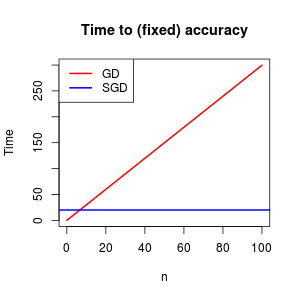
\includegraphics[scale=0.55]{comparison}
	\end{figure}

			
\end{frame}

\begin{frame}
	\frametitle{SGD is widely used in industry}
	If a Silicon Valley press release uses any of the following phrases...
	\begin{itemize}
		\item \small ``Neural networks''
		\item ``Machine learning''
		\item ``AI'' 
	\end{itemize}

	...SGD probably is involved. Example: Google's \textbf{AlphaGo} program.

	\begin{figure}[b]
	\centering
	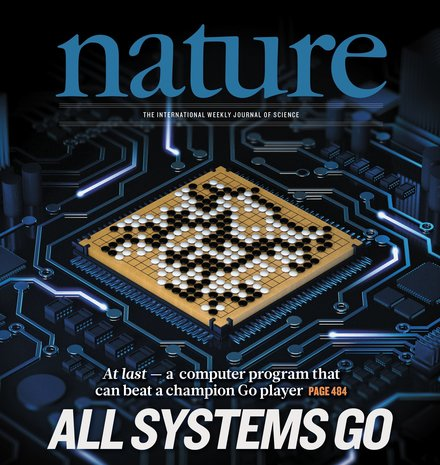
\includegraphics[scale=0.25]{go}
	\end{figure}

\end{frame}

\end{document}


